\subsection{Motivation for Hash Tables}
\begin{intuition}
    In many computer science problems, we need to efficiently solve the \textbf{dictionary problem}, which consists of operations like:
    \vspace{1em}

    \textbf{Dictionary operations:}
    \begin{itemize}
        \item Insert
        \item Search
        \item Delete
        \item Sort (won't be covered in hashing)
    \end{itemize}
    \vspace{1em}

    For instance, storing Social Insurance Numbers (SINs) is an example of a scenario where fast retrieval is essential.

    There are two basic approaches:
    \begin{itemize}
        \item \textbf{Array:} Offers \( O(1) \) search but wastes a lot of memory.
        \item \textbf{Linked List:} Memory efficient $O(n)$ but time inefficient with \( O(n) \) search.
    \end{itemize}

    \customFigure[0.75]{00_Images/HTM.png}{Difference between array and linked lists.}
    \vspace{1em}

    Hash tables offer a tradeoff between these two approaches. Instead of wasting memory like arrays or sacrificing time efficiency like linked lists, hash tables use a hash function to map keys to positions in a table, resolving collisions with methods such as chaining or open addressing.
\end{intuition}

\subsection{Introduction to Hash Tables}

\subsubsection{Definition}
\begin{definition}
A \textbf{hash table} uses a hash function to map keys from the universe of keys \( U \) to positions in an array of size \( m \) called buckets. 
\begin{itemize}
    \item The key is stored in the appropriate bucket. 
    \item The number of keys stored is \( n \).
    \item The \textbf{load factor} \( \alpha \) is given by: $\alpha = \frac{n}{m}, \quad 0 < \alpha \leq 1$
    \begin{itemize}
        \item Expect $n \leq m$ so the places to store in the array is bigger than the number of keys to store in $n$.
    \end{itemize}
\end{itemize}
\end{definition}

\subsubsection{Hash Function}
\begin{definition}
A \textbf{hash function} \( h(\text{key}) \) is used to convert a key into a numeric value, which is then used to index the array. 
\begin{itemize}
    \item i.e. Maps a key in $U$ to an index from $0$ to $m-1$.
    \item A good hash function minimizes collisions, where two or more keys are assigned to the same index.
\end{itemize}
\end{definition}

\begin{example}
    \customFigure[0.75]{00_Images/C.png}{Collisions happening between D and E and also C and F}
    \begin{itemize}
        \item The array goes from $0$ to $m-1$ (i.e. array of size $m$)
        \item The hash function maps the keys from $U$ to the bucket.
        \item Use a linked list for collisions (i.e. resolutions by chaining).
        \item \textbf{Worst-case:} May all hash to the same index. So what constitutes a good hash function. 
    \end{itemize}
\end{example}

\subsection{Method for designing hash functions}
\subsubsection{Modulo}
\begin{definition}
    The modulo operator, denoted as \( \mod \), returns the remainder when one number is divided by another. Specifically, for two integers \( a \) and \( b \), the expression \( a \mod b \) yields the remainder when \( a \) is divided by \( b \).
\end{definition}

\subsubsection{Division Method}
\begin{definition}
    The \textbf{division method} computes the hash as:
    \[
    h(\text{key}) = \text{key} \mod m
    \]
    \begin{itemize}
        \item \( m \) is typically a prime number. 
    \end{itemize}
\end{definition}

\begin{intuition}
    To avoid clustering, \( m \) should be a prime number not too close to a power of 2. This ensures better distribution of keys across the table. 
    \begin{itemize}
        \item Using powers of 2 for \( m \) can lead to poor distributions and clustering. It only considers the lower-order bits of the key, leading to many collisions as different keys may have identical lower bits.

    \end{itemize}
\end{intuition}

\begin{example}
    For example, let \( m = 7 \) and the keys be: 12, 44, 13, 88.
    \[
    h(12) = 12 \mod 7 = 5
    \]
    \[
    h(44) = 44 \mod 7 = 2
    \]
    \[
    h(13) = 13 \mod 7 = 6
    \]
    \[
    h(88) = 88 \mod 7 = 4
    \]

    The array table would be:

    \[
    \begin{array}{|c|c|}
    \hline
    \text{Index} & \text{Key} \\
    \hline
    0 &  \\
    1 &  \\
    2 & 44 \\
    3 &  \\
    4 & 88 \\
    5 & 12 \\
    6 & 13 \\
    \hline
    \end{array}
    \]
\end{example}

\subsubsection{Multiplication Method}
\begin{definition}
The \textbf{multiplication method} computes the hash as:
\[
h(\text{key}) = \left\lfloor m \cdot ((\text{key} \cdot A) \mod 1) \right\rfloor
\]
\begin{itemize}
    \item \( A = \frac{\sqrt{5} - 1}{2} \), the golden ratio, is used to spread keys more evenly. 
    \item $m = 2^p$ are good values.  
\end{itemize}
\end{definition}

\begin{example}
        The multiplication method computes the hash function as: 
    \[
    h(\text{key}) = \lfloor m \cdot ((\text{key} \cdot A) \mod 1) \rfloor
    \]
    where \( A \approx 0.6180339887 \) and \( m = 16 \).

    For example, with keys 123, 456, 789, 102, the hash values are:

    \[
    \begin{array}{|c|c|}
    \hline
    \text{Index} & \text{Key} \\
    \hline
    0 & 123, 102 \\
    1 &  \\
    2 &  \\
    3 &  \\
    4 &  \\
    5 &  \\
    6 &  \\
    7 &  \\
    8 &  \\
    9 &  \\
    10 & 789 \\
    11 &  \\
    12 &  \\
    13 & 456 \\
    14 &  \\
    15 &  \\
    \hline
    \end{array}
    \]    
\end{example}

\subsubsection{Universal Hashing}
\begin{definition}
In \textbf{universal hashing}, a family of hash functions \( H = \{ h_1, h_2, h_3, \ldots \} \) is randomly chosen from. The key advantage is that it reduces the probability of collisions between specific sets of keys.
\end{definition}

\subsection{Resolution by Chaining}
\begin{definition}
\textbf{Chaining} is a method of resolving collisions by maintaining a linked list at each bucket. If two or more keys hash to the same index, they are stored in the same linked list.
\end{definition}

\begin{intuition}
Chaining is simple and can easily handle cases where multiple keys collide by inserting them into the linked list of the corresponding bucket. The downside is that it can lead to increased search time if the linked lists become long.
\end{intuition}

\subsection{Resolution by Open Addressing}

\begin{definition}
\textbf{Open addressing} resolves collisions by probing for the next available slot in the table. 
\begin{itemize}
    \item Instead of maintaining a list of keys at each bucket, each key is placed directly in the table, and a probing sequence is followed if collisions occur.
\end{itemize}
\end{definition}

\subsubsection{Probing Methods}
\begin{definition}
    \begin{itemize}
        \item \textbf{Linear Probing:} Probe and insert next element:
        
        \[
        L_0 = h(\text{key})
        \]
        
        If bucket is full (i.e. collision), then we check the next slot in the table until an empty one is found (i.e. reprobe)
        \[
        L_{j+1} = (L_j + 1) \mod m
        \]
        \begin{itemize}
            \item However, linear probing can lead to \textbf{clustering}, where groups of keys form large contiguous blocks in the array.
        \end{itemize}
        \customFigure[0.5]{00_Images/Cl.png}{Clustering}
    
        \item \textbf{Double Hashing:} Using two hash functions to avoid clustering. If a collision occurs at index \( i_0 \):
        \[
        L_1 = h_1(\text{key}) 
        \]
        The next probe location is computed by:
        \[
        L_{j+1} = (L_j + h_2(\text{key})) \mod m
        \]
        \begin{itemize}
            \item This results in better distribution of keys across the table and reduces clustering.
        \end{itemize}
    \end{itemize}
\end{definition}

\begin{example}
    Example of linear probing:
    \textbf{Given:}
    \begin{itemize}
        \item Hash table size, $m = 7$
        \item Probe step size, $c = 3$
        \item Hash function: $h(\text{key}) = \text{key} \mod 7$
        \item Keys to insert: \{14, 8, 21, 10\}
    \end{itemize}
    
    \textbf{Insertion of Keys:}
    \begin{enumerate}
        \item \textbf{Insert 14}:
           \[
           h(14) = 14 \mod 7 = 0
           \]
           Place 14 at index 0.
    
        \item \textbf{Insert 8}:
           \[
           h(8) = 8 \mod 7 = 1
           \]
           Place 8 at index 1.
    
        \item \textbf{Insert 21}:
           \[
           h(21) = 21 \mod 7 = 0
           \]
           Collision at index 0 (occupied by 14).  
           Perform linear probing with step size 3:
           \[
           \text{Next index} = 0 + 3 = 3
           \]
           Place 21 at index 3.
    
        \item \textbf{Insert 10}:
           \[
           h(10) = 10 \mod 7 = 3
           \]
           Collision at index 3 (occupied by 21).  
           Perform linear probing with step size 3:
           \[
           \text{Next index} = 3 + 3 = 6
           \]
           Place 10 at index 6.
    \end{enumerate}
    
    \textbf{Current Hash Table:}
    
    \[
    \begin{array}{|c|c|}
    \hline
    \text{Index} & \text{Value} \\
    \hline
    0 & 14 \\
    1 & 8 \\
    2 & - \\
    3 & 21 \\
    4 & - \\
    5 & - \\
    6 & 10 \\
    \hline
    \end{array}
    \]
    
    \textbf{Deletion of Keys:}
    \begin{enumerate}
        \item \textbf{Remove 21}:
           \[
           h(21) = 0
           \]
           Check index 0: Not 21.  
           Perform linear probing:
           \[
           \text{Next index} = 0 + 3 = 3
           \]
           Find 21 at index 3, remove it, and place a tombstone at index 3.
    
        \item \textbf{Remove 10}:
           \[
           h(10) = 3
           \]
           Check index 3: Tombstone.  
           Perform linear probing:
           \[
           \text{Next index} = 3 + 3 = 6
           \]
           Find 10 at index 6 and remove it.
    \end{enumerate}
    
    \textbf{Final Hash Table:}
    
    \[
    \begin{array}{|c|c|}
    \hline
    \text{Index} & \text{Value} \\
    \hline
    0 & 14 \\
    1 & 8 \\
    2 & - \\
    3 & \text{Tombstone} \\
    4 & - \\
    5 & - \\
    6 & \text{Tombstone} \\
    \hline
    \end{array}
    \]
    
    \textbf{Explanation:} Tombstones are used in open addressing to indicate that an element was removed from that position. If a tombstone is found during probing, the search continues, ensuring that other elements inserted with probing can still be located.
    
\end{example}

\subsection{Load Factor in Open Addressing and Chaining}
\begin{definition}
    The expected search time (i.e. expected number of probes) depends on the load factor \( \alpha \) and the probing method used:
    \begin{itemize}
        \item Deteriorates as $\alpha$ increases because it increases the number of collisions (i.e. more probes required).
    \end{itemize}

    \begin{itemize}
        \item \textbf{Linear Probing:} 
        \[
        \text{\# Probes} = \frac{1}{2} \left( 1 + \frac{1}{1 - \alpha} \right)
        \]
        \item \textbf{Double Hashing:} 
        \[
        \text{\# Probes} = \frac{1}{\alpha} \ln \left( \frac{1}{1 - \alpha} \right) \approx O(1) \text{ if } n<m
        \]
        \item \textbf{Chaining:}
        \[
            \text{\# Probes} = 1 + \frac{\alpha}{2}
            \]
    \end{itemize}
    \begin{itemize}
        \item \textbf{Note:} The number of collisions is the number of probes.
    \end{itemize}
\end{definition}

\begin{intuition}
    Chaining (blue), linear probing (red), double hashing (green)

    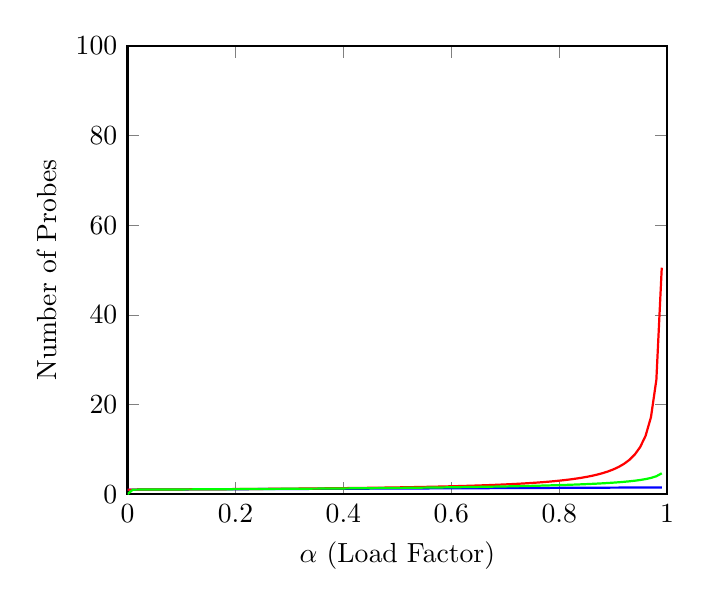
\begin{tikzpicture}
        \begin{axis}[
            xlabel={$\alpha$ (Load Factor)},
            ylabel={Number of Probes},
            xmin=0, xmax=1,
            ymin=0, ymax=100,
            domain=0:0.99,
            samples=100,
            thick
        ]
        
        % Chaining
        \addplot[
            color=blue,
            solid,
        ]{1 + x/2};
    
        % Linear Probing
        \addplot[
            color=red,
            solid,
        ]{0.5*(1 + 1/(1-x))};
    
        % Double Hashing
        \addplot[
            color=green,
            solid,
        ]{(1/x)*ln(1/(1-x))};
        \end{axis}
    \end{tikzpicture}    
\end{intuition}
